\documentclass[conference]{IEEEtran} % default font size: 10pt
\usepackage{times,microtype}

\usepackage{graphicx}
\usepackage[caption=false]{subfig}
\graphicspath{{images/}}

\usepackage{amsmath,amssymb,mathtools}

\usepackage[inline]{enumitem}

\renewcommand{\vec}[1]{\boldsymbol{#1}}
\DeclarePairedDelimiter{\abs}{\lvert}{\rvert}
\DeclarePairedDelimiter{\norm}{\lVert}{\rVert}

% numbers option provides compact numerical references in the text.
\usepackage[numbers]{natbib}
\usepackage{multicol}
\usepackage[bookmarks=true]{hyperref}

\pdfinfo{ % TODO: update info below
   /Author (Homer Simpson)
   /Title  (Robots: Our new overlords)
   % /CreationDate (D:20101201120000)
   /Subject (Robots)
   /Keywords (Robots;Overlords)
}

\begin{document}

% TODO: paper title
\title{Is minimalistic MPC based on centroidal dynamics enough to race complex vehicles?}

% You will get a Paper-ID when submitting a pdf file to the conference system TODO: update info below
\author{Author Names Omitted. Paper-ID [add your ID here]}

%\author{\authorblockN{Michael Shell}
%\authorblockA{School of Electrical and\\Computer Engineering\\
%Georgia Institute of Technology\\
%Atlanta, Georgia 30332--0250\\
%Email: mshell@ece.gatech.edu}
%\and
%\authorblockN{Homer Simpson}
%\authorblockA{Twentieth Century Fox\\
%Springfield, USA\\
%Email: homer@thesimpsons.com}
%\and
%\authorblockN{James Kirk\\ and Montgomery Scott}
%\authorblockA{Starfleet Academy\\
%San Francisco, California 96678-2391\\
%Telephone: (800) 555--1212\\
%Fax: (888) 555--1212}}


% avoiding spaces at the end of the author lines is not a problem with
% conference papers because we don't use \thanks or \IEEEmembership


% for over three affiliations, or if they all won't fit within the width
% of the page, use this alternative format:
%
%\author{\authorblockN{Michael Shell\authorrefmark{1},
%Homer Simpson\authorrefmark{2},
%James Kirk\authorrefmark{3},
%Montgomery Scott\authorrefmark{3} and
%Eldon Tyrell\authorrefmark{4}}
%\authorblockA{\authorrefmark{1}School of Electrical and Computer Engineering\\
%Georgia Institute of Technology,
%Atlanta, Georgia 30332--0250\\ Email: mshell@ece.gatech.edu}
%\authorblockA{\authorrefmark{2}Twentieth Century Fox, Springfield, USA\\
%Email: homer@thesimpsons.com}
%\authorblockA{\authorrefmark{3}Starfleet Academy, San Francisco, California 96678-2391\\
%Telephone: (800) 555--1212, Fax: (888) 555--1212}
%\authorblockA{\authorrefmark{4}Tyrell Inc., 123 Replicant Street, Los Angeles, California 90210--4321}}


\maketitle

% ----------------------------------------------------------------------------------------

\begin{abstract}
	MPC is often used to control in real time various systems and processes in the 
	chemical, mechanical and electrical fields. Here we focus on its use in autonomous 
	driving. In particular, we investigate whether a minimalistic MPC based on a 
	point mass model is able to drive a complete multibody vehicle model.
	Then we propose a method, called MPC offset-free, useful to compensate
	the differences between the MPC internal model and the driven vehicle.
\end{abstract}

\IEEEpeerreviewmaketitle

\section{Introduction}
Autonomous driving is one of the most discussed and actual topic in research and industrial fields. Here, we focus our attention on autonomous race car. In particular, in literature, three different approaches are employed in order to compute real-time control input for an autonomous car. 
In the first one the control of the vehicle is realized with a deep dense neural network, which is trained with recorded vehicle data to represent the vehicle's dynamic behaviour \textbf{cita{1-2-3}}. In the second approach a model predictive control (MPC) solves at each sampling instant, a finite horizon open-loop control problem, using the current state of the system as the initial state; the optimization yields an optimal control sequence and the first control in this sequence is applied as an input \textbf{cita{4-5-6}}. The last method is a mix of the previous approaches, in this case a learning model predictive control (LNMPC) is used in order to find optimal control and
to learn the system model and the disturbance acting on it through the data from the previous trajectories \textbf{cita{7-8-9}}.  


In our work, we start from the classical MPC approach, and we employ a minimalistic MPC, hence a very simplified vehicle model is used as MPC internal model in order to reduce computational time. 
After that the offset-free theory developed in \textbf{cita{Pannocchia}}, is implemented in order to compensate the differences between the MPC model and the driven vehicle. 
%\textcolor{gray}{\lipsum[1]}



% ----------------------------------------------------------------------------------------

\section{Proposed approach} % TODO: if the method has a name, use it here as section title


\subsection{Model of the simulated vehicle}


\subsection{MPC internal model}

In order to race the fully-fledged vehicle we build an MPC dynamic model from first principles which strives to be as minimalistic as possible for maximum computational efficiency yet able to capture the fundamentals of vehicle dynamics. To this sake, a point-mass model is devised, embodying the dynamics of the center of mass (CoM) of the full model.
This model has 5 DoFs and, worthily enough, it employs the very same basic parameters of the full vehicle, such as: mass, aerodynamic coefficients, grip and power limits for braking and traction phases. These are usually readily available even for a complex vehicle.

Control inputs are the longitudinal force $F_{x}$, and the angular acceleration along the vertical axes $r_p = dr/dt$, where $r$ is the yaw rate~\footnote{It is worth remarking that the apparent nonsense of introducing the yaw rate for a point mass is resolved if one thinks of its dynamics written in the body-fixed reference frame. This justifies the introduction of a yaw rate for the point mass which is the same as the body-fixed reference frame's yaw rate.}.

The steering angle, needed to control the simulated vehicle, can be extracted by assuming that
\begin{equation}
\delta = \alpha_{1} + \beta_1 = F_{y_{11}}/C_\alpha + (v + ra_1)/u
\end{equation}
where, exploiting the same notation in~\citet{Guiggiani2018}, $C_\alpha$ is the cornering stiffness of the front tire and $a_1$ is the distance between the Centre of Mass (CoM) and the front axle.
Tire slip angles $\alpha_{1i}$ and vehicle slip angles $\beta_{1i}$ are assumed equal for each wheel $i=1, 2$ of the same axle, hence $\alpha_{11} = \alpha_{12} = \alpha_{1}$ and $\beta_{11} = \beta_{12} = \beta_{1}$.
%
Front wheel lateral forces $F_{y_{1i}}$ are estimated within the steady-state assumption, leading to $F_{y_{11}} = F_{y_{12}} = F_{y}a_2/(2l)$.
$F_{y}$, included as an algebraic state, summarizes the total lateral force acting on the vehicle model. Then, $a_2$ is the distance between the CoM and the rear axle and $l$ is the wheelbase.

\subsection{Spatial formulation}

The race track, assumed planar, is modelled through the parametric 2D curve
\begin{equation}
\mathcal C(\alpha) = \{ \vec x (\alpha) = [x(\alpha), y(\alpha)]^T \in \mathbb{R}^2 : \alpha \in [\alpha_0, \alpha_f] \}
\end{equation}
%
that identifies the road centerline (aka track spine), and the 1D curve $\mathcal W(\alpha)$ that specifies the track width.
With reference to Figure~\ref{fig:scheme_frenet_serret_refsys}, the \emph{curve parameter} $\alpha$ uniquely selects a point $\vec F = \vec x(\alpha)$ that defines the origin of the \emph{Frenet-Serret frame} $\mathcal F = \{ \vec F, (\vec t, \vec p) \}$ with unit tangent and normal vectors $\vec t$ and $\vec p$ of $\mathcal C$ at point $\vec F$.
%
The vehicle reference system $\mathcal V = \{ \vec G, (\vec i, \vec j) \}$ can be expressed with the aid of the moving frame $\mathcal F$ with a \emph{lateral displacement} $e_p$ along the track normal direction $\vec p$ and the \emph{heading error} $e_\psi$.
% = \psi_f - \psi_v
In order to maintain $\mathcal F$ side-by-side with $\mathcal V$, the Frenet-Serret system has to proceed together with the vehicle: this leads to a relation between vehicle and Frenet-Serret velocities that ultimately imposes a bound between time and $\alpha$ increments.

%The final formulation of the vehicle model dynamics, % TODO: ref to standard formulation, if previously exposed
%extended with lateral displacement, heading error and transposed in spatial domain is
%
%\begin{equation} \left\{
%\begin{aligned}
%u_{,\alpha} &= \frac{\norm{\hat{\vec x}_{,\alpha}}}{s_p} \left[ \frac{1}{m} (F_{x} - X_a) + vr \right] \\
%v_{,\alpha} &= \frac{\norm{\hat{\vec x}_{,\alpha}}}{s_p} \left[ \frac{F_{y}}{m} - ur \right] \\
%r_{,\alpha} &= \frac{\norm{\hat{\vec x}_{,\alpha}}}{s_p} r_{p}  \\
%e_{p,\alpha} &= \frac{\norm{\hat{\vec x}_{,\alpha}}}{s_p} \left[ u \sin{e_\psi} + v \cos{e_\psi} \right] \\
%e_{\psi,\alpha} &= \norm{\hat{\vec x}_{,\alpha}} \left( \frac{r}{s_p} - k \right),
%\end{aligned} \right.
%\label{eq:vehicle_state_update_alpha_domain}
%\end{equation}
%%
%where the notation $u_{,\alpha} = \frac{du}{d \alpha}$ has been used to shorten derivative notations.

\begin{figure}[htb] \centering
	%  \subfloat[]
	%    {\includegraphics[width=.5\linewidth]{example-image-a}} % NOTE: this needs `mwe' package
	%  \quad
	\subfloat[]{\includegraphics[width=.4\linewidth]{scheme_frenet_serret_refsys}
		\label{fig:scheme_frenet_serret_refsys}}
	\caption{(\textbf{a}) vehicle pose respect to the Frenet-Serret reference system identified on the track curve.}
	\label{fig:scheme_frenet_serret}
\end{figure}


\subsection{OCP problem formulation}

The centroidal dynamics is formulated in spatial domain instead of the time, and the \emph{direct collocation} is used to transform the \emph{Optimal Control Problem} (OCP) into a \emph{Non-Linear Program} (NLP). The NLP is coded in a scripting environment using the Matlab interface to the open-source CasADi framework written by \citet{Andersson2019}, which provides building
blocks to efficiently formulate and solve large-scale optimization problems, and solved through IPOPT~\cite{Wachter2006}.

The OCP is formulated with the goal of finding the optimal control sequence necessary to minimize the travel time of the next $l_N$ meters of the track ahead of the vehicle.

\subsection{Offset-free MPC}
\label{sec:offsetfree}


% ----------------------------------------------------------------------------------------

\section{Preliminary results}
The MPC controller is tested on the Indianapolis oval racing track. In particular, three different simulations are performed:
\begin{enumerate*}[label=(\roman*)]
	\item lap-time simulation with MPC controller,
	\item lap-time simulation with MPC controller in which the aerodynamic drag is neglected in the MPC internal model,
	\item lap-time simulation with offset-free MPC,
\end{enumerate*}
where the aerodynamic drag is estimated through the technique explained in \ref{sec:offsetfree}.

Solutions in terms of controlled vehicle trajectories and inputs are compared, focusing on the entry phase of the first curve.

\begin{figure}[htb] \centering
    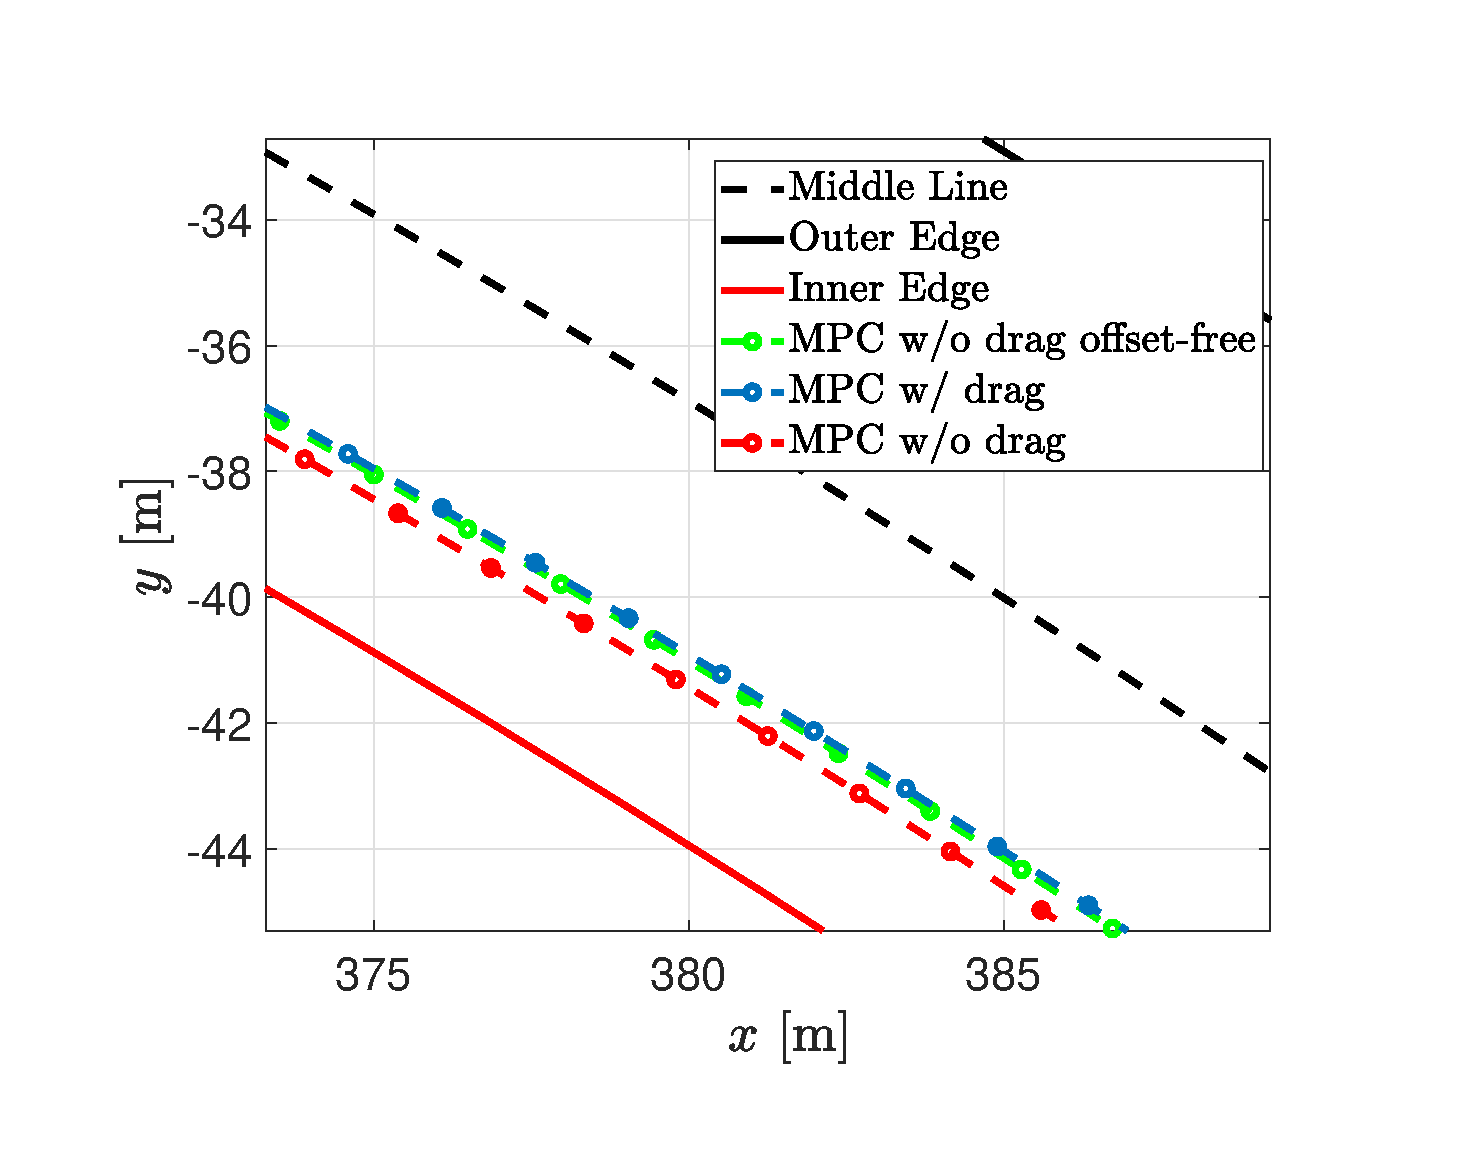
\includegraphics[width=1.\linewidth]{Trajectories2}
	\caption{Trajectories comparison between lap simulation with MPC (blue), MPC offset-free (green), MPC without drag (red)}
	\label{fig:Trajectories2}
\end{figure}

\begin{figure}[htb] \centering
	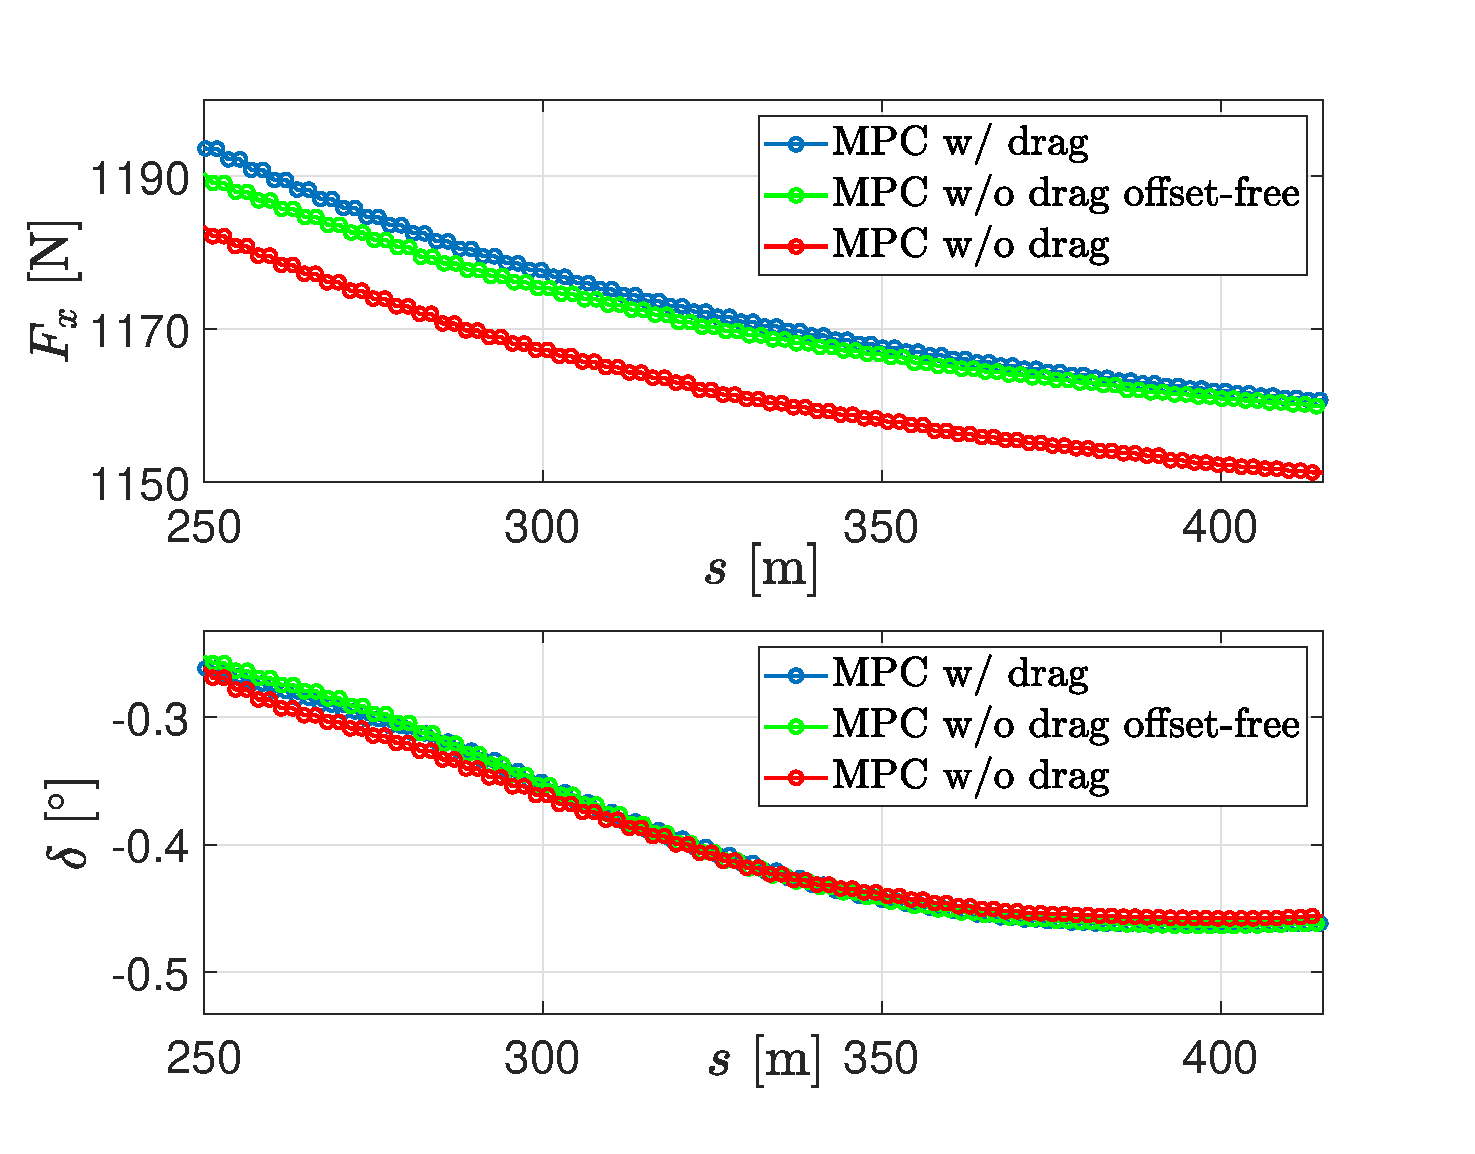
\includegraphics[width=1.\linewidth]{steer_fx} % FIXME: what is the unit on the abscissa? Minutes (min)?
	\caption{Comparison between control inputs, longitudinal force (top), steering angle of the front wheel (bottom), obtained with MPC (blue), MPC offset-free (green) and MPC without drag (red)}
	\label{fig:steer_fx}
\end{figure}

Figures.\ref{fig:Trajectories2} - \ref{fig:steer_fx} highlight how MPC with drag and MPC offset-free are capable to drive the Adams vehicle in a practically identical way, with a lap-time difference of $6.5$ms. Instead, if the aerodynamic drag is not modelled inside the MPC, the controller is not able to maintain the real vehicle on the track: in fact the simulation fails on the entry phase of the second curve.

%\textcolor{gray}{\lipsum[5]}

% ----------------------------------------------------------------------------------------

\section{Conclusion}
The minimalistic MPC based solely on the vehicle centroidal dynamics seems enough to race complex vehicle counterpart.
% NOTE: 'In particular' or 'However'? The following sentence seems a limitation
In particular, parameters of the MPC model such as mass, aerodynamic coefficients or power limits, have to be equal to those of the driven car: in this way the point-mass model can be considered as a condensed model of the complex vehicle itself.

Nevertheless, the offset-free technique is a powerful and efficient addendum that allows to relax even further the internal model. It is also forgiving enough to adjust some uncertain yet fundamental parameters of the complex vehicle in a convenient way at run time.
As a proof of concept, an internal model agnostic of the aerodynamic drag has shown to dramatically benefit from the estimation of the drag force through the disturbance state $d$.

Further developments to the MPC internal model, as well as new approaches to the estimation of the steer angle, can lead to drive the full vehicle in conditions even closer to handling limits.
\label{sec:conclusion}


% ----------------------------------------------------------------------------------------

%% Use plainnat to work nicely with natbib.
\bibliographystyle{plainnat}
\bibliography{references}

\end{document} 